\subsection{Komparator}
En analog komparator er et kredsløb, der sammenligner en input spænding eller strøm med en eller flere reference spændinger eller strømme. Komparatorens output går fra den ene mætningsgrænsen til den anden, når det negative input af operationsforstærkeren passere igennem 0 V. Dette betyder at ved en input spænding på mere end tærskel niveauet vil output spændingen opnå negativ mætningsgrad. Omvendt vil en input spænding, som er lavere end tærskel niveauet vil output spændingen opnå positiv mætningsgrad \fxnote{skriv hvorfor dette sker rent teknisk}.  Den simpleste komparator er en operations forstærker. Det kan være fordelagtig at placerer modstanden R1 ved input signalet, som det kan ses på \figref{komparator} da dette minimere overstyringen \fxnote{Et bedre ord end overstyring} af operations forstærkeren.  Når inputtet ved en simpel komparator når tærskel niveauet og der er støj på inputtet, så kan output signalet svinge vildt. Dette kan midlertidig undgås ved at tilføje to modstande, R2 og R3, som det kan ses på \figref{komparator}.  \cite{webster2009}
\begin{figure}[H]
\centering
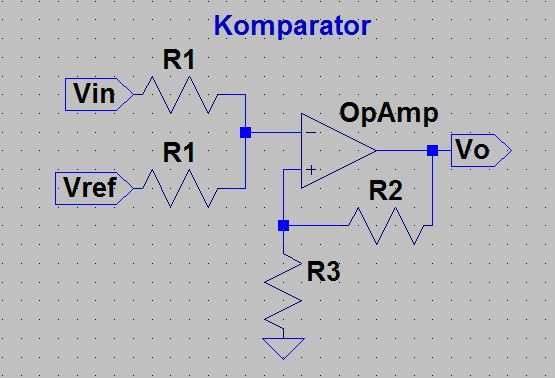
\includegraphics[scale=0.7]{figures/cProblemloesning/Komparator.JPEG}
\caption{En simpel komparator, der har fået tilføjet R2 og R3 for at undgå svingninger i output signalet.}
\label{komparator}
\end{figure}
